\subsection*{Hjørner}\label{subsec:corner}
Et hjørne kan defineres som et område i og omkring et punkt, der har to dominerede kantretninger og derved kan lokaliseres i et billede ud fra en kvantificeret fortolkning af dette. \\ 
I figur \ref{app} ses tre udvalgte interessepunkter, placeret på forskellige strukturer i samme scene, hvor interessepunkterne beskrives af en blå cirkel omkring punktet. For at forstå, hvorfor punkter placeret på hjørner er gode interessepunkter, er mulige korrespondancer for de givne interessepunkter illustreret.
\begin{enumerate}[label=\alph*]
\item{Interessepunktet er placeret på et fladt området, hvor intensiteten er ens for hele området. Punktet vil have mange mulige korresponderende punkter.}
\item{Interessepunktet er lokaliseret på en kant. Punktet vil have flere mulige korresponderende punkter på den tilsvarende kant i den anden figur.}
\item{Interessepunktet er lokaliseret på et hjørne. Det ses at kun ét andet punkt i modsvarende scene er identisk med dette.}
\end{enumerate}
\begin{figure}[H]
    \centering
    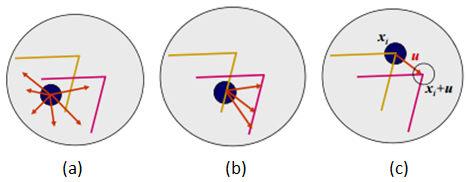
\includegraphics[width=0.55\textwidth]{fig/37.png}
    \vspace{-1em}   
    \begin{center}    
    \caption{\textcolor{gray}{\footnotesize \textit{
 }}}
    \label{app}
     \end{center}
    \vspace{-2.7em}  
  \end{figure}  
\noindent
Ovenstående definition viser at punkter placeret på hjørner er unikke. Hjørner kan som nævnt udvælges i billederne pga. de dominerende kantretninger i og omkring punktet, hvilket medfører store intensitetsskift i området omkring et hjørne.